\section*{Глава 2. Проектирование веб-приложения}
\addcontentsline{toc}{section}{Глава 2. Проектирование веб-приложения}
\stepcounter{section}

\subsection{Анализ целевой аудитории}

Целевая аудитория разрабатываемого веб-приложения включает три основные группы пользователей:
покупателей, менеджеров магазина и администраторов системы.

\textbf{Покупатель} использует приложение для просмотра каталога цифровой электроники,
поиска и фильтрации товаров, изучения характеристик, добавления товаров в корзину и
оформления заказа. Для данной группы важны понятная навигация по категориям, быстрый
поиск по названию и характеристикам, корректное отображение цены и наличия товара.

\textbf{Менеджер} отвечает за обработку заказов, изменение их статусов, проверку состава
покупки и коммуникацию с клиентом. Для менеджера особенно важны список новых заказов,
информация о покупателе, составе заказа, общей сумме и текущем состоянии выполнения.

\textbf{Администратор} управляет товарным каталогом, категориями, пользователями и правами
доступа. Его рабочие сценарии связаны с добавлением новых моделей электроники, редактированием
цен, описаний, изображений, складских остатков и характеристик товаров.

\subsection{Описание функциональности приложения}

Проектируемое приложение должно поддерживать основные сценарии интернет-магазина цифровой
электроники. Покупатель просматривает каталог, выбирает категорию, применяет фильтры,
открывает карточку товара, добавляет товар в корзину и оформляет заказ. После оформления
заказ сохраняется в системе, а пользователь может просмотреть его состояние в истории покупок.

Менеджер просматривает поступившие заказы, уточняет их состав и изменяет статус обработки.
Администратор добавляет и редактирует товары, категории и учетные записи сотрудников.

К основным функциональным модулям относятся:
\begin{itemize}
    \item каталог товаров с категориями цифровой электроники;
    \item карточка товара с описанием, ценой, изображением, характеристиками и остатком;
    \item поиск, фильтрация и сортировка товаров;
    \item корзина покупателя;
    \item оформление и хранение заказов;
    \item личный кабинет покупателя с историей покупок;
    \item административный интерфейс управления товарами, категориями и заказами;
    \item разграничение прав доступа для покупателей, менеджеров и администраторов.
\end{itemize}

\subsection{Проектирование модели данных}

Модель данных веб-приложения строится вокруг сущностей, характерных для интернет-магазина:
пользователей, категорий, товаров, корзины, заказов и позиций заказа. Между ними существуют
устойчивые связи: товар относится к категории, заказ принадлежит пользователю, а каждая
позиция заказа ссылается на конкретный товар.

Структура основных таблиц представлена в таблице~2.1.

\begin{longtable}{|p{3.2cm}|p{4cm}|p{7cm}|}
    \caption{Основные сущности модели данных} \label{tab:data_model} \\
    \hline
    \textbf{Сущность} & \textbf{Ключевые поля} & \textbf{Назначение} \\ \hline
    \endfirsthead
    \tabcont{\ref{tab:data_model}}
    \textbf{Сущность} & \textbf{Ключевые поля} & \textbf{Назначение} \\ \hline
    \endhead
    \hline
    \endfoot
    \hline
    \endlastfoot

    Пользователь & id, username, email, password, role & Хранение учетных записей покупателей, менеджеров и администраторов \\ \hline
    Категория & id, name, slug, description & Группировка товаров по разделам каталога \\ \hline
    Товар & id, category\_id, name, description, price, stock, image, specifications & Хранение информации о цифровой электронике и ее характеристиках \\ \hline
    Корзина & id, user\_id, created\_at & Временное хранение выбранных пользователем товаров \\ \hline
    Позиция корзины & id, cart\_id, product\_id, quantity & Связь товара с корзиной и выбранным количеством \\ \hline
    Заказ & id, user\_id, status, total\_price, delivery\_address, created\_at & Фиксация оформленной покупки и состояния обработки \\ \hline
    Позиция заказа & id, order\_id, product\_id, quantity, price & Хранение состава заказа и цены товара на момент покупки \\ \hline
\end{longtable}

На рисунке~2.1 представлена ER-диаграмма базы данных,
отражающая сущности системы и связи между ними.

\begin{figure}[H]
    \centering
    
\includegraphics[width=0.95\textwidth]{er_diagram}
    \caption{ER-диаграмма базы данных интернет-магазина}
    \label{fig:er_diagram}
\end{figure}

\subsection{Разработка макетов страниц и пользовательских сценариев}

Интерфейс приложения проектируется с учетом разделения на публичную часть и административную
панель. Публичная часть включает главную страницу, каталог, страницу категории, карточку товара,
корзину, страницу оформления заказа и личный кабинет. Административная часть содержит списки
товаров, категорий и заказов, а также формы создания и редактирования записей.

Основной пользовательский сценарий покупателя выглядит следующим образом:
\begin{enumerate}
    \item Пользователь открывает каталог магазина цифровой электроники (см. рисунок 2.2).
    \item Выбирает категорию или находит товар через поиск.
    \item Изучает карточку товара и добавляет его в корзину.
    \item Проверяет состав корзины (см. рисунок 2.3) и переходит к оформлению заказа.
    \item Указывает контактные данные и адрес доставки.
    \item Подтверждает заказ и отслеживает его статус в личном кабинете.
\end{enumerate}

\begin{figure}[H]
    \centering
    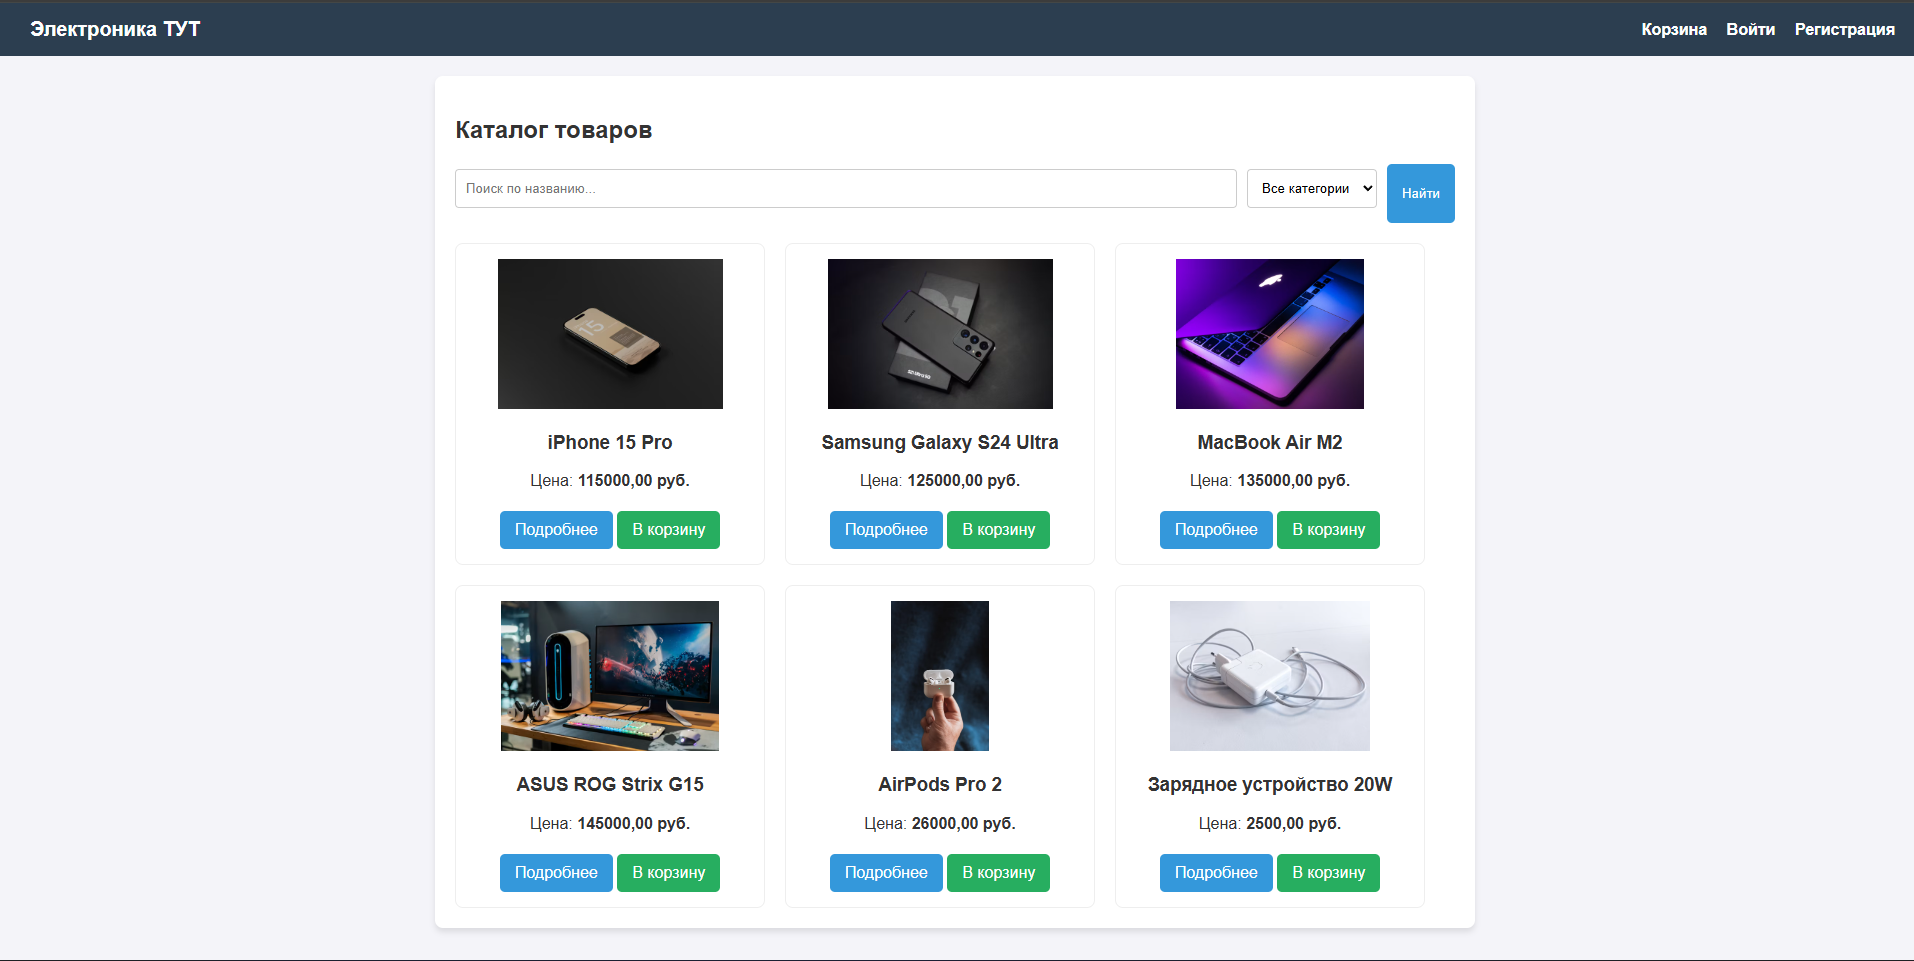
\includegraphics[width=0.95\textwidth]{images/main_website.png}
    \caption{Главная страница веб-приложения}
    \label{fig:main_website}
\end{figure}

\begin{figure}[H]
    \centering
    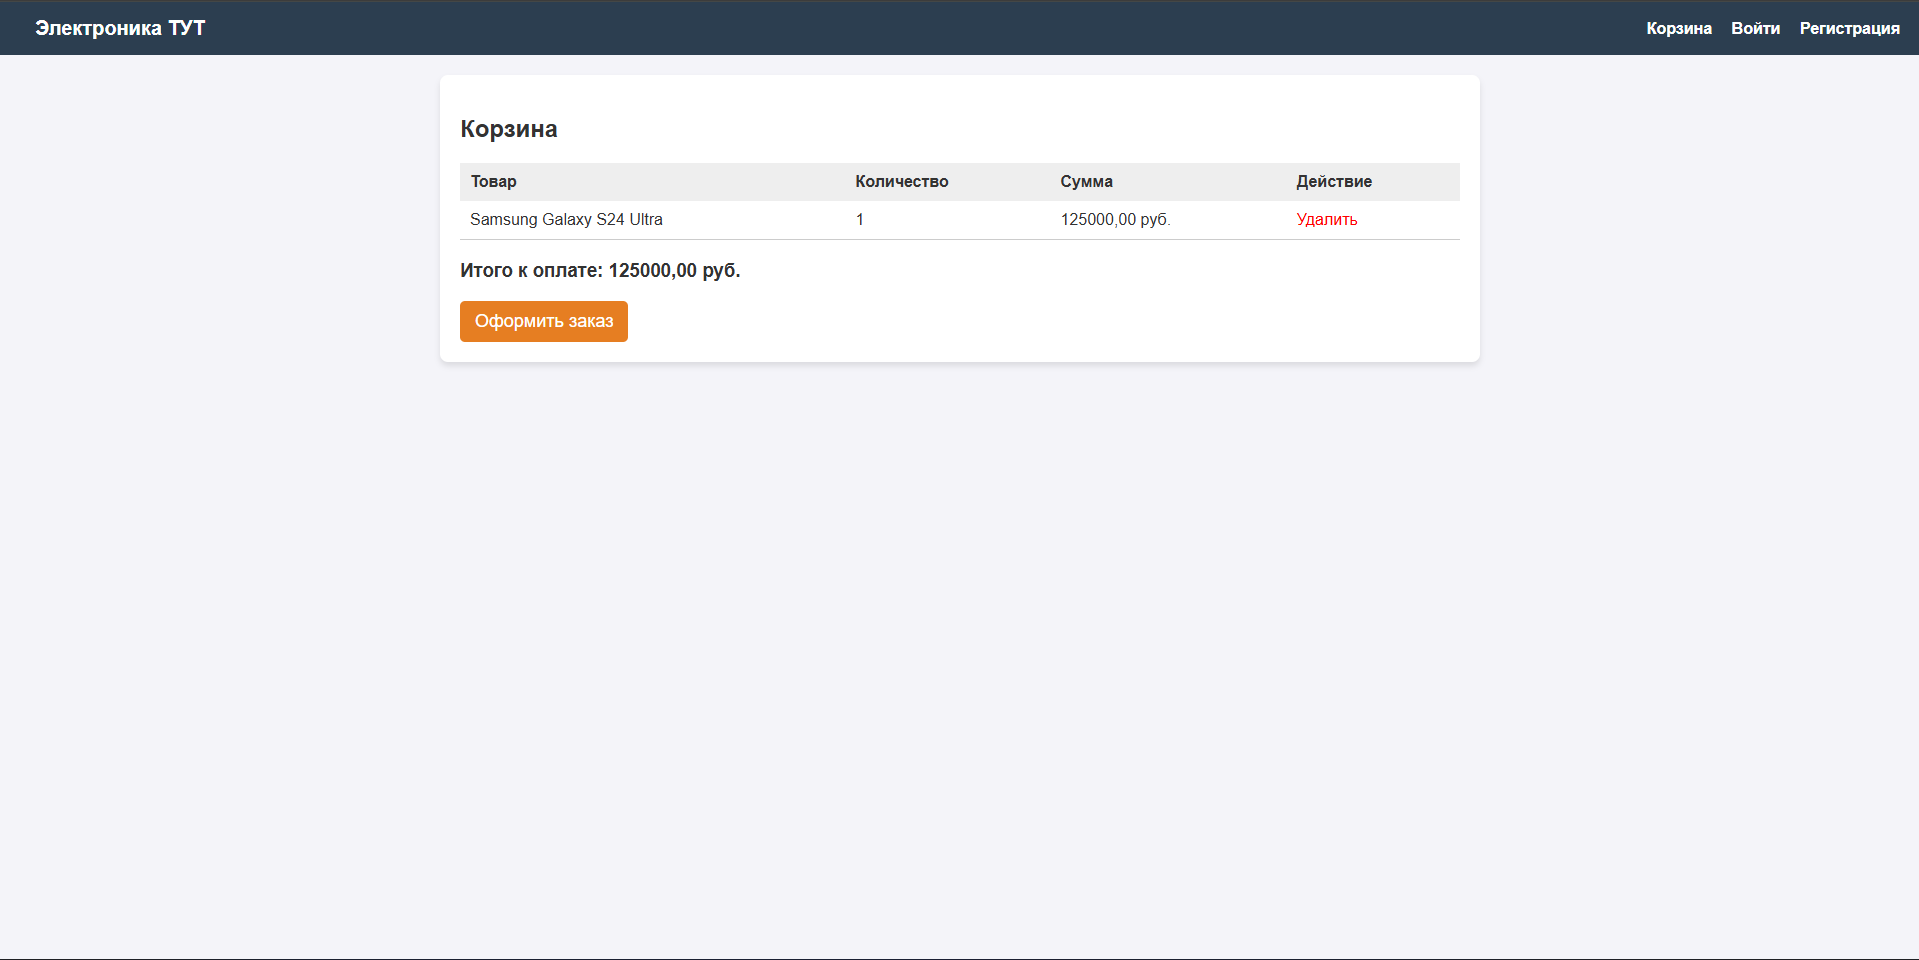
\includegraphics[width=0.95\textwidth]{images/корзина.png}
    \caption{Страница корзины пользователя}
    \label{fig:cart}
\end{figure}

Такое проектирование позволяет заранее определить состав страниц, структуру данных и
основные точки взаимодействия пользователя с системой.
